\section{Boltzmann マシン}
\subsection{Boltzmann マシン}
(Boltzmann machine)
\subsection{制限 Boltzmann マシン}
(Restricted Boltzmann machine) 
(cf.) \url{http://deeplearning.net/tutorial/rbm.html}
データの読み込み
\lstinputlisting[language=julia]{./text/energy-based-model/boltzmann-machine/003.jl}
\lstinputlisting[language=julia]{./text/energy-based-model/boltzmann-machine/004.jl}
\lstinputlisting[language=julia]{./text/energy-based-model/boltzmann-machine/005.jl}
\begin{figure}[ht]
	\centering
	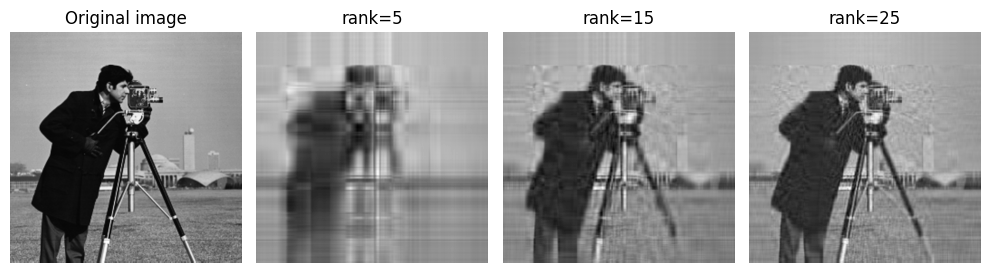
\includegraphics[scale=0.8, max width=\linewidth]{./fig/solve-credit-assignment-problem/linear-network-learning-dynamics/cell005.png}
	\caption{cell005.png}
	\label{cell005.png}
\end{figure}
\lstinputlisting[language=julia]{./text/energy-based-model/boltzmann-machine/006.jl}
\lstinputlisting[language=julia]{./text/energy-based-model/boltzmann-machine/007.jl}
離散の観測変数(visible variable) $\mathbf{v}$, 潜在変数(hidden variable) $\mathbf{h}$とする.各ユニットの値は$\{0, 1\}$の2値 (binary)である.

エネルギー関数を


\begin{equation}
E_\theta(\mathbf{v}, \mathbf{h})=-\mathbf{b}^T \mathbf{v} - \mathbf{c}^T \mathbf{h} + \mathbf{v}^T \mathbf{W} \mathbf{h}
\end{equation}


とする.ただし,$\theta=\{\mathbf{W}, \mathbf{b}, \mathbf{c}\}$
\lstinputlisting[language=julia]{./text/energy-based-model/boltzmann-machine/009.jl}
シグモイド関数を


\begin{equation}
\sigma(x) = \frac{1}{1+\exp(-x)}
\end{equation}


とする.
\subsubsection{訓練データで学習}

\begin{align}
p_\theta(\mathbf{h}|\mathbf{v})&=\prod_i p_\theta(h_i=1|\mathbf{v})=\prod_i \sigma(c_i + W_i \mathbf{v})\\
p_\theta(\mathbf{v}|\mathbf{h})&=\prod_j p_\theta(v_j=1|\mathbf{h})=\prod_j \sigma(b_j + W_j^T \mathbf{h})
\end{align}
\lstinputlisting[language=julia]{./text/energy-based-model/boltzmann-machine/012.jl}
二項分布 (bernoulli distribution)のサンプリングには2通りある.\jl{1.0f0}を乗じているのはBool変数からFloatへの変換のため.詳細はtips.
テストデータで確認
\lstinputlisting[language=julia]{./text/energy-based-model/boltzmann-machine/015.jl}
\lstinputlisting[language=julia]{./text/energy-based-model/boltzmann-machine/016.jl}
\begin{figure}[ht]
	\centering
	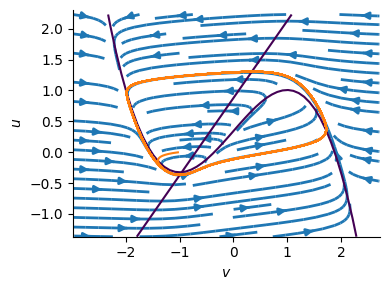
\includegraphics[scale=0.8, max width=\linewidth]{./fig/neuron-model/fhn/cell016.png}
	\caption{cell016.png}
	\label{cell016.png}
\end{figure}
\lstinputlisting[language=julia]{./text/energy-based-model/boltzmann-machine/017.jl}
\lstinputlisting[language=julia]{./text/energy-based-model/boltzmann-machine/018.jl}
\begin{figure}[ht]
	\centering
	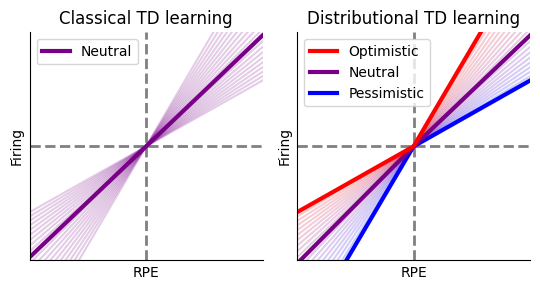
\includegraphics[scale=0.8, max width=\linewidth]{./fig/bayesian-brain/quantile-expectile-regression/cell018.png}
	\caption{cell018.png}
	\label{cell018.png}
\end{figure}
エネルギーの変化を見る
\lstinputlisting[language=julia]{./text/energy-based-model/boltzmann-machine/020.jl}
\begin{figure}[ht]
	\centering
	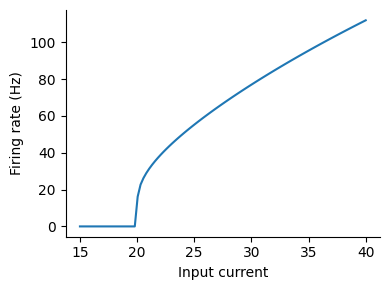
\includegraphics[scale=0.8, max width=\linewidth]{./fig/neuron-model/lif/cell020.png}
	\caption{cell020.png}
	\label{cell020.png}
\end{figure}
受容野の可視化
\lstinputlisting[language=julia]{./text/energy-based-model/boltzmann-machine/022.jl}
\begin{figure}[ht]
	\centering
	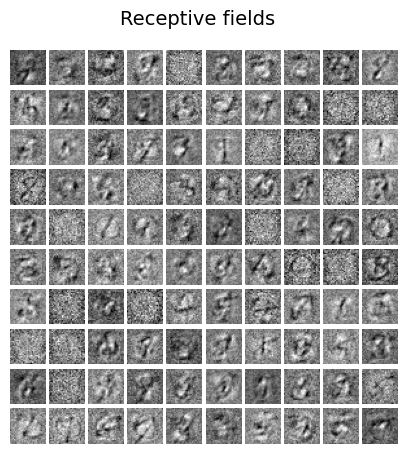
\includegraphics[scale=0.8, max width=\linewidth]{./fig/energy-based-model/boltzmann-machine/cell022.png}
	\caption{cell022.png}
	\label{cell022.png}
\end{figure}
